\documentclass{beamer}
\usepackage[english]{babel}
\usepackage[latin1]{inputenc}
\usepackage{amsmath,amsfonts,amssymb}
\usepackage{units}
\usepackage{color}
\usepackage{enumitem}
\usepackage{braket}
\usepackage{bbm}
\usepackage{graphicx}


\usetheme{Frankfurt}
\usecolortheme{seahorse}
\usecolortheme{rose}

\newcommand\blfootnote[1]{%
  \begingroup
  \renewcommand\thefootnote{}\footnote{#1}%
  \addtocounter{footnote}{-1}%
  \endgroup
}

\DeclareMathOperator{\e}{e}
\setlist[itemize,1]{label={\textcolor{lightblue}{$\bullet$}}}
\setlist[itemize,2]{label={\textcolor{lightblue}{$\Rightarrow$}}}

\definecolor{lightblue}{rgb}{.43137254,.48235294,.54509803}


\title{Band structure studies for graphene and modified graphene structures}

\author{Dirk Hornung}
\date{09.03.2014}

\begin{document}

\begin{frame}[plain]
	\titlepage
\end{frame}

\section*{Structure}
\subsection*{1}

%\begin{frame}
%	\frametitle{Bandstructure}
%		\begin{itemize}
		 
		
		
	
%		 \end{itemize}
%\end{frame}


%\begin{frame}
 % \frametitle{Derivation: \(\alpha(Im(\epsilon))\)}
  %\begin{itemize}
    %\item {\textcolor{lightblue}{N. Osakabe et al., Phy Rev. A \textbf{34} 2, 815 (1986)}}
    %\includegraphics[width=0.5\linewidth]{Abbildungen/Versuchsaufbau.png}
    %\includegraphics[width=0.3\linewidth]{Abbildungen/Feld_Torus.png}
  %\end{itemize}

%\end{frame}

\begin{frame}
	\frametitle{Structure}
	\begin{itemize}
		\item Introduction
		\vspace{0.3cm}
		\item Carbon materials
		\vspace{0.3cm}
		\item Tight binding fit
		\vspace{0.3cm}
		\item DFT results
	\end{itemize}
\end{frame}

\section{Introduction}

	\subsection*{1}
		\begin{frame}
			\frametitle{Introduction}
			\centering
			\begin{columns}[T] % align columns
				\begin{column}{.48\textwidth}
					\includegraphics[width=1.2\textwidth]{figures/grapheneManuscripts.png}
				\end{column}%
				\hfill%
				\begin{column}{.48\textwidth}
					\includegraphics[width=\textwidth]{figures/Graphen.jpg}
				\end{column}%
			\end{columns}
			\blfootnote{\textsuperscript{Left} Data from 'http://www.arxiv.org' }
			\blfootnote{\textsuperscript{Right} Image from article 'http://de.wikipedia.org/wiki/Graphen'}			
		\end{frame}
		
		\subsection*{2}
		\begin{frame}
			\frametitle{Introduction}
			\centering
			\begin{itemize}
				\item thickness of one atom
				\vspace{0.3cm}
				\item transparent
				\vspace{0.3cm}
				\item strongest material
				\vspace{0.3cm}
				\item best heat conductivity
				\vspace{0.3cm}
				\item electric conductivity equal to copper
				\vspace{0.3cm}
				\item electrons show relativistic behavior 
			\end{itemize}
		\end{frame}


\section{Carbon materials}
	\subsection*{1}
	
		\begin{frame}
			\frametitle{The carbon atom}
			\centering
			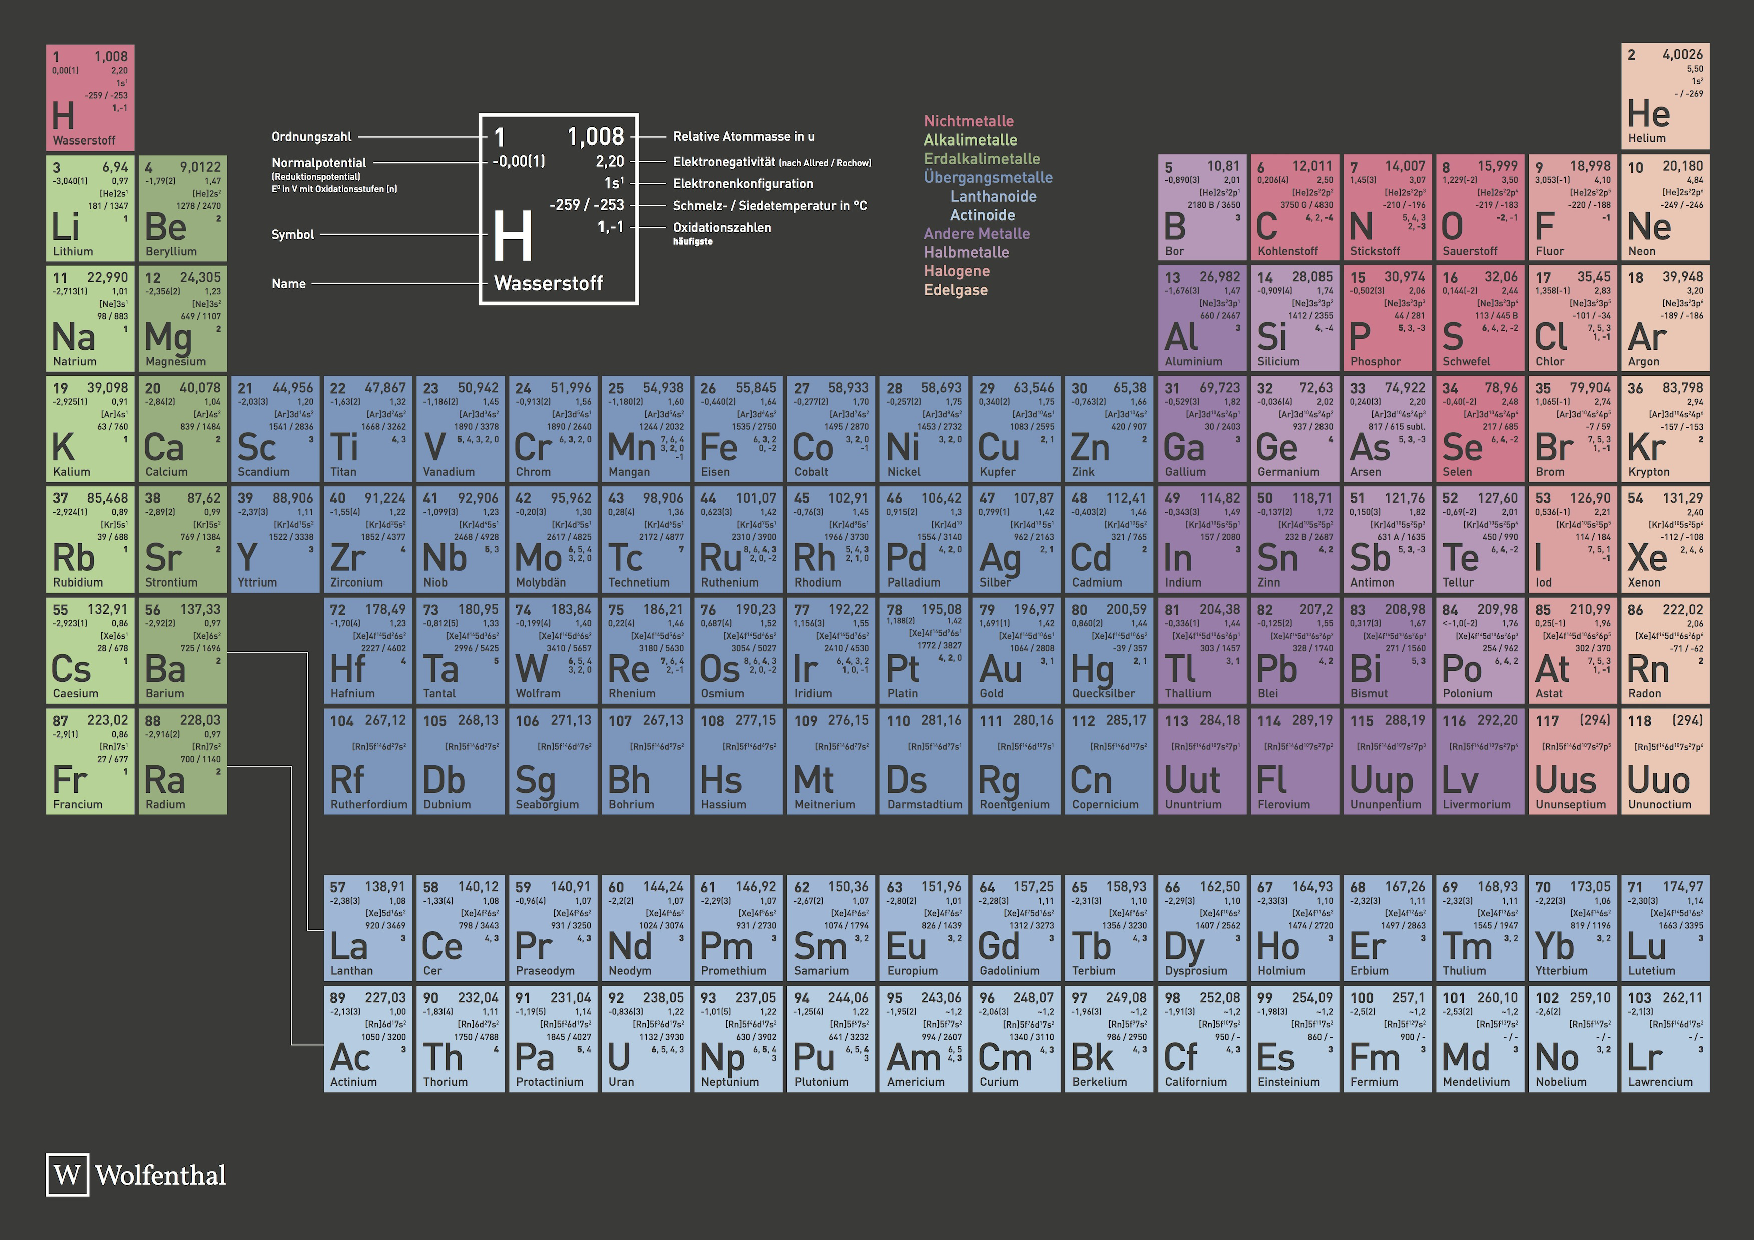
\includegraphics[width=0.8\textwidth]{figures/periodicTable.PDF}	
			\begin{equation}
				\text{ground state: } 1s^2 2s^2 2p^2
			\end{equation}
			\blfootnote{Image from 'http://www.wolfenthal.de/drucken' }
		\end{frame}

	\subsection*{2}
		\begin{frame}
			\frametitle{sp\textsuperscript{2}-hybridization}
			\centering
			\includegraphics[width=0.8\textwidth]{figures/carbonHybridization2.png}
			\begin{align}
				| sp_1^2 \rangle &= \tfrac{1}{\sqrt{3}} | 2s \rangle - \sqrt{\tfrac{2}{3}} | 2p_y \rangle, \\
				| sp_2^2 \rangle &= \tfrac{1}{\sqrt{3}} | 2s \rangle + \sqrt{\tfrac{2}{3}} (\tfrac{\sqrt{3}}{2} |2 p_x \rangle + \tfrac{1}{2} | 2p_y \rangle), \\
				|sp_3^2 \rangle &= - \tfrac{1}{\sqrt{3}} | 2s \rangle + \sqrt{\tfrac{2}{3}} ( - \tfrac{\sqrt{3}}{2} | 2p_x \rangle + \tfrac{1}{2} | 2 p_y \rangle)
			\end{align}	
			\blfootnote{Image from Noel, Jean and Oliver, Mark : 'Introduction of the Physical Properties of Graphen' }		
		\end{frame}

	\subsection*{3}
		\begin{frame}
			\frametitle{Graphene lattice}
			\centering
			\includegraphics[width=0.7\textwidth]{figures/grapheneLattice.png}
			\begin{align}
				\boldsymbol{\delta_1} = \frac{a}{2} (\sqrt{3} \vec{e_y} - \vec{e_z}) && \boldsymbol{\delta_1} = - \frac{a}{2} (\sqrt{3} \vec{e_y} + \vec{e_z}) && \boldsymbol{\delta_3} = a \vec{e_z}.
			\end{align}
			\begin{align}
				\vec{a_1} = \sqrt{3} a \vec{e_y} && \vec{a_2} =  \frac{\sqrt{3}a}{2} (\vec{e_y} + \sqrt{3} \vec{e_z}).
			\end{align}			
		\end{frame}

	\subsection*{4}
		\begin{frame}
			\frametitle{Graphene Lattice}
			\centering
			\begin{columns}[T] % align columns
				\begin{column}{.48\textwidth}
					\includegraphics[width=\textwidth]{figures/grapheneBrillouin.png}
				\end{column}%
				\hfill%
				\begin{column}{.48\textwidth}
					\begin{align}
						\vec{g_1} = \frac{2\pi}{\sqrt{3}a} (\vec{e_y} - \frac{\vec{e_z}}{\sqrt{3}}) \\
						 \vec{g_2} = \frac{4 \pi}{3a} \vec{e_z} \\
						 \pm \vec{K} = \pm \frac{4 \pi}{3 \sqrt{3}a}\vec{e_y}
					\end{align}
				\end{column}%
			\end{columns}				
		\end{frame}

\section{Tight binding fit}

	\subsection*{1}
		\begin{frame}
			\frametitle{Nearest neighbor analytical solution}
			\begin{equation}
				\epsilon_k^{\pm \pi} = t'f_{nnn}(\vec k) \pm t\sqrt{3 + f_{nnn}(\vec k)}
			\end{equation}
			with
			\begin{equation}
				f_{nnn}(\vec k) = 2\cos(\sqrt{3} k_x a ) + 4\cos(\frac{3}{2} k_y a)\cos(\frac{\sqrt{3}}{2}k_x a).
			\end{equation}			
		\end{frame}

	\subsection*{2}
		\begin{frame}
			\frametitle{Electronic dispersion in the honeycomb lattice}
			\centering
			\includegraphics[width=\textwidth]{figures/tightBinding3dplot.png}
		\end{frame}

	\subsection*{3}
		\begin{frame}
			\frametitle{Pi bands}
			\underline{Band structure of graphene}
			\includegraphics[width=\textwidth]{figures/tightBindingPiGraphene.pdf}
		\end{frame}

	\subsection*{4}
		\begin{frame}
			\frametitle{Pi bands}
			\underline{Separation}
			\includegraphics[width=\textwidth]{figures/piPlusMinus.png}	
		\end{frame}
		
	\subsection*{4}
		\begin{frame}
			\frametitle{Calculated parameters}
			\begin{table}[h]
				\centering
				\begin{equation}
					\sigma = \sqrt{\left( \epsilon_{k}^{\pm \pi} - \epsilon_{FPLO} \right)^2},
				\end{equation}
				\vspace{0.4cm}
				\begin{tabular}{cccc}
				     & t & t' & $\sigma$ \\
					\midrule
					 $\pi_+$ & 1.54 & -1.09 & 272.89 \\
					 $\pi_-$ & 1.35 & 0.59 & 80.52 \\
					\bottomrule
				\end{tabular}
				\caption{The tight binding parameters t, t' and the plot variance $\sigma$.}
			\end{table}
		\end{frame}

	\subsection*{5}
		\begin{frame}
			\frametitle{Pi plus fit}
			\includegraphics[width=\textwidth]{figures/fit1.png}
		\end{frame}

	\subsection*{6}
		\begin{frame}
			\frametitle{Pi minus fit}
			\includegraphics[width=\textwidth]{figures/fit2.png}
		\end{frame}


\section{DFT results}
	
	\subsection*{1}
		\begin{frame}
			\frametitle{Graphene}
			\underline{Vesta structure}
			\begin{columns}[T] % align columns
				\begin{column}{.48\textwidth}
					\includegraphics[width=\textwidth]{figures/graphite.png}
				\end{column}%
				\hfill%
				\begin{column}{.48\textwidth}
					\includegraphics[width=0.8\textwidth]{figures/graphene.png}
				\end{column}%
			\end{columns}
		\end{frame}

	\subsection*{2}
		\begin{frame}
			\frametitle{Graphene}
			\underline{Weighted band structure}
			\includegraphics[width=\textwidth]{figures/GrapheneNew/bweights.pdf}
		\end{frame}

	\subsection*{3}
		\begin{frame}
			\frametitle{Graphene}
			\underline{DOS}
			\includegraphics[width=\textwidth]{figures/GrapheneNew/dos.pdf}
		\end{frame}
	
	\subsection*{4}
		\begin{frame}
			\frametitle{Modifying graphene}
			\underline{Vesta structures}
			\begin{columns}[T] % align columns
				\begin{column}{.28\textwidth}
					\centering
					\includegraphics[width=\textwidth]{figures/GrapheneBor1_20A.png} \\
					Unite cell length : \textbf{2.687} $\boldsymbol{\AA}$
				\end{column}%
				\hfill%
				\begin{column}{.28\textwidth}
					\centering
					\includegraphics[width=\textwidth]{figures/GrapheneNitrogen1_20A.png} \\
					Unite cell length : \textbf{2.477} $\boldsymbol{\AA}$
				\end{column}%
				\hfill%
				\begin{column}{.28\textwidth}
					\centering
					\includegraphics[width=\textwidth]{figures/GrapheneSilicium1_20A.png} \\
					Unite cell length : \textbf{3.112} $\boldsymbol{\AA}$
				\end{column}%
			\end{columns}
		\end{frame}
		
	\subsection*{5}
		\begin{frame}
			\frametitle{Boron modified graphene}
			\underline{Weighted band structure}
			\includegraphics[width=\textwidth]{figures/Bor1R/bweights.pdf}
		\end{frame}

	\subsection*{6}
		\begin{frame}
			\frametitle{Boron modified graphene}
			\underline{DOS}
			\includegraphics[width=\textwidth]{figures/Bor1R/dos.pdf}
		\end{frame}

	\subsection*{7}
		\begin{frame}
			\frametitle{Boron modified graphene}
			\underline{Stability}
			\begin{center}
				Total energy of \textbf{-62.881 eV} \\
				\begin{equation}
					BC^{layer} \xrightarrow{\Delta E} C_2^{layer}
				\end{equation}
				$\boldsymbol{\Delta}$ \textbf{E = -13.287 eV}
			\end{center}
		\end{frame}
		
	\subsection*{8}
		\begin{frame}
			\frametitle{Nitrogen modified graphene}
			\underline{Weighted band structure}
			\includegraphics[width=\textwidth]{figures/Nitrogen1R/bweights.pdf}
		\end{frame}

	\subsection*{9}
		\begin{frame}
			\frametitle{Nitrogen modified graphene}
			\underline{DOS}
			\includegraphics[width=\textwidth]{figures/Nitrogen1R/dos.pdf}
		\end{frame}
		
	\subsection*{10}
		\begin{frame}
			\frametitle{Nitrogen modified graphene}
			\underline{Stability}
			\begin{center}
				Total energy of \textbf{-92.743 eV} \\
				\begin{equation}
					NC^{layer} \xrightarrow{\Delta E} C_2^{layer}
				\end{equation}
				$\boldsymbol{\Delta}$ \textbf{E = 16.575 eV}
			\end{center}
		\end{frame}
		
	\subsection*{11}
		\begin{frame}
			\frametitle{Silicon modified graphene}
			\underline{Weighted band structure}
			\includegraphics[width=\textwidth]{figures/Silicon1R/bweights.pdf}
		\end{frame}
		
	\subsection*{12}
		\begin{frame}
			\frametitle{Silicon modified graphene}
			\underline{Stability}
			\begin{center}
				Total energy of \textbf{-327.459 eV} \\
				\begin{equation}
					SiC^{layer} \xrightarrow{\Delta E} C_2^{layer}
				\end{equation}
				$\boldsymbol{\Delta}$ \textbf{E = 251.291 eV}
			\end{center}
		\end{frame}

	\subsection*{13}
		\begin{frame}
			\frametitle{Silicon modified graphene}
			\underline{DOS}
			\includegraphics[width=\textwidth]{figures/Silicon1R/dos.pdf}
		\end{frame}
	
	\subsection*{14}
		\begin{frame}
			\vspace{2cm}
			\centering
			\underline{Thank you}
		\end{frame}

\end{document}
